
\section{Thực nghiệm}

\begin{frame}{Dataset}
	
%	$x^{2} \in \mathbb{R}^{x \times y}$

\begin{columns}
	\begin{column}{0.6\textwidth}
		ZeroEGGs Dataset \cite{ghorbani2023zeroeggs}:
		
		\begin{itemize}
			\item Bao gồm 67 đoạn độc thoại của diễn viên motion capture nữ
			\item Độ dài toàn bộ tập dữ liệu là 135 phút.
			\item Bao  gồm 6 cảm xúc: Happy,  Sad, Neutral, Old, Relaxed, Angry
		\end{itemize}
		%	\includepdf[pages=-]{images/EmotionPCA.pdf}
		\includegraphics[width=\linewidth]{EmotionPCA.pdf}
	\end{column}
	
	\begin{column}{0.4\textwidth}
		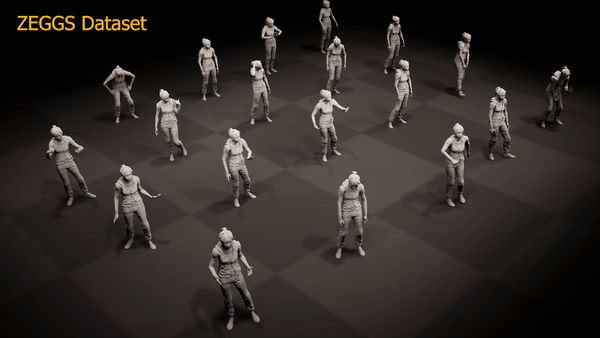
\includegraphics[width=\linewidth]{ZEGGsData}
	\end{column}
\end{columns}
\end{frame}



\begin{frame}{Training Process}
	Toàn bộ quá trình học trong 1 ngày với tham số sau:
\begin{itemize}
	\item $T = 1000$
	\item Sử dụng Card Nvidia 3090
	\item Chia dataset thành tỷ lệ: $8:1:1$ cho lần lượt: tập training, testing và validation.
	\item Learning rate: $3 \times 10^{-5}$
	\item 384 batch size với 300000 samples.
	\end{itemize}
	
	\textbf{Mã nguồn chương trình}: \hyperlink{https://github.com/hmthanh/OHGesture}{hmthanh/OHGesture}
\end{frame}

\begin{frame}{Emotion Demo}
	\begin{figure}
	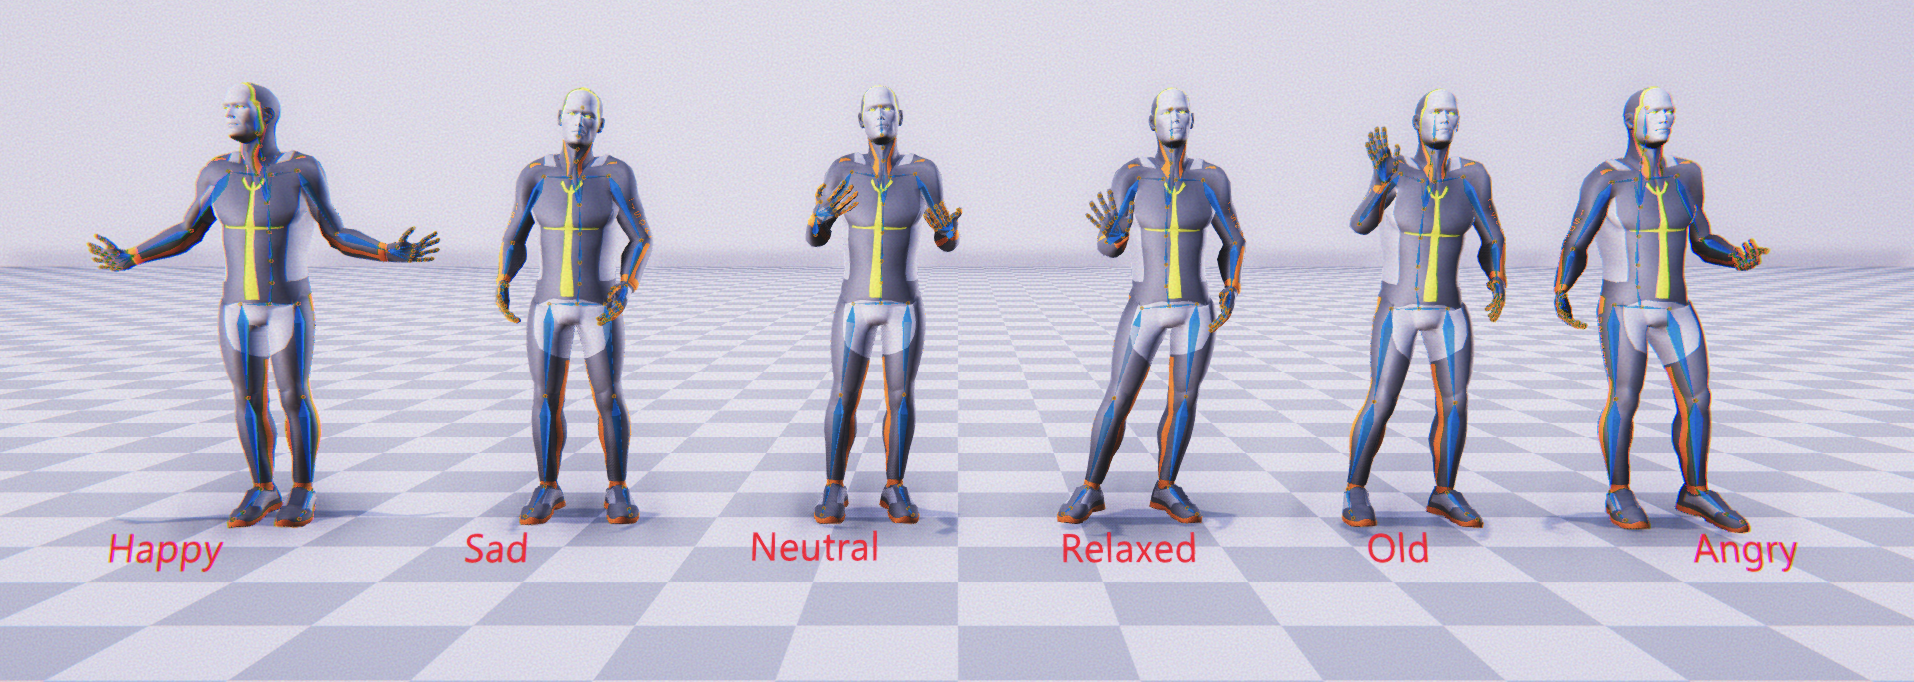
\includegraphics[width=\textwidth]{EmotionAnimation}
\end{figure}
\end{frame}